%%%%%%%%%%%%%%%%%%%%%%%%%%%%%%%%%%%%%%%%%%%%%%%%%%
%%%%%%%%%%%%%%%%%%%%%%%%%%%%%%%%%%%%%%%%%%%%%%%%%%
%%
%% Based one the "beamer-greek-two" template provided 
%% by the Laboratory of Computational Mathematics, 
%% Mathematical Software and Digital Typography, 
%% Department of Mathematics, University of the Aegean
%% (http://myria.math.aegean.gr/labs/dt/)
%%
%% Adapted by John Liaperdos, October-November 2014
%% (ioannis.liaperdos@gmail.com)
%%
%% Last update: 26/11/2014
%%
%%%%%%%%%%%%%%%%%%%%%%%%%%%%%%%%%%%%%%%%%%%%%%%%%%
%%%%%%%%%%%%%%%%%%%%%%%%%%%%%%%%%%%%%%%%%%%%%%%%%%
%%
\PassOptionsToPackage{unicode}{hyperref}
\PassOptionsToPackage{naturalnames}{hyperref}
\documentclass[11pt]{beamer} 
%\usepackage[spanish]{babel}
\usepackage[utf8]{inputenc}
\usepackage[italicdiff]{physics}
\usepackage{empheq}
\usepackage{pgf}
\usepackage[absolute,overlay]{textpos}
%\usepackage[texcoord,grid,gridunit=mm,gridcolor=red!30,subgridcolor=green!30]{eso-pic}

%%% FONT SELECTION %%%%%%%%%%%%%%%%%
%%% we choose a sans font %%%%%%%%%%
%\usepackage{kmath,kerkis} 
%\usepackage[default]{gfsneohellenic} 
\usefonttheme{professionalfonts}
%%%%%%%%%%%%%%%%%%%%%%%%%%%%%%%%%%%%

\usepackage{color}
\usepackage{amsmath}
\usepackage{amssymb}

\usepackage{epstopdf}
\usepackage{graphicx}
\graphicspath{{./figures/}}

%%
% load TEI-Pel - specific layout
\usepackage{mylayout}
\setTeipelLayout{draft}% options: "draft", "newlogo"

%%%%%%%%%%%%%%%%%%%%%%%%%%%%%%%%%%%%%%%%%%%%%%%%%%%%%%%%%%%%
% Thesis Info %%%%%%%%%%%%%%%%%%%%%%%%%%%%%%%%%%%%%%%%%%%%%%
%%%%%%%%%%%%%%%%%%%%%%%%%%%%%%%%%%%%%%%%%%%%%%%%%%%%%%%%%%%%
	% title
		\title[Estructura estelar de objetos compactos]{Estructura estelar de objetos compactos con una ecuación de estado numérica}	
	% author 
    % (In the mandatory argument "{}", separate multiple
    % authors with "\and" - use "\\" for better author name formatting
    % in the title page. Names in latin should be formatted using the
    % \textlatin{name} macro. In the optional argument "[]" include all
	% author names, with no "\and" or text formatting macros.)
	% Example: 
    %\author[Κ. Δημητρίου Albert Einstein]{Κωνσταντίνος Δημητρίου \and \textlatin{Albert Einstein}}
		\author[David Ramos]{David Ramos}
	% supervisor	
		\supervisor{Director}{Luis Núñez}
%%%%%%%%%%%%%%%%

\begin{document}

% typeset front slides
	\typesetFrontSlides

%%%%%%%%%%%%%%%%
% Your Slides Start here:

\section{Formación y evolución estelar}


\begin{frame}{Formación estelar}
    \begin{figure}
    \centering
    \begin{minipage}{.5\textwidth}
        \centering
        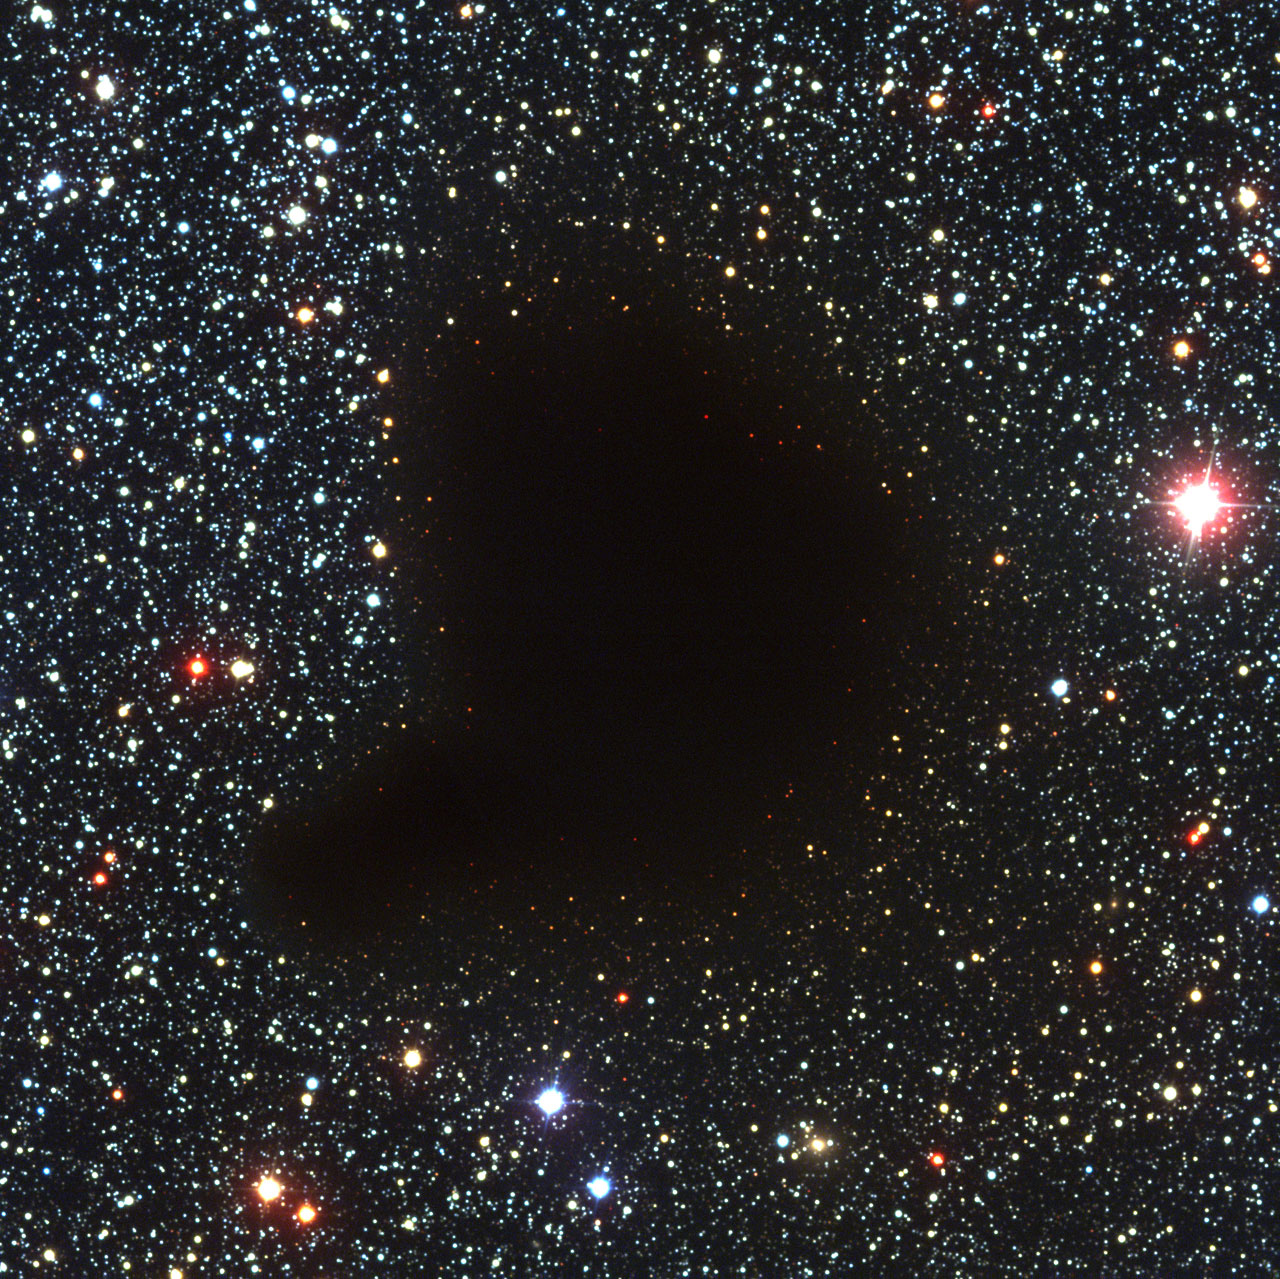
\includegraphics[width=.9\linewidth]{barnard.jpg}
        \captionof{figure}{Barnard 68. Fuente: ESO}
    \end{minipage}%
    \begin{minipage}{.5\textwidth}
        \centering
        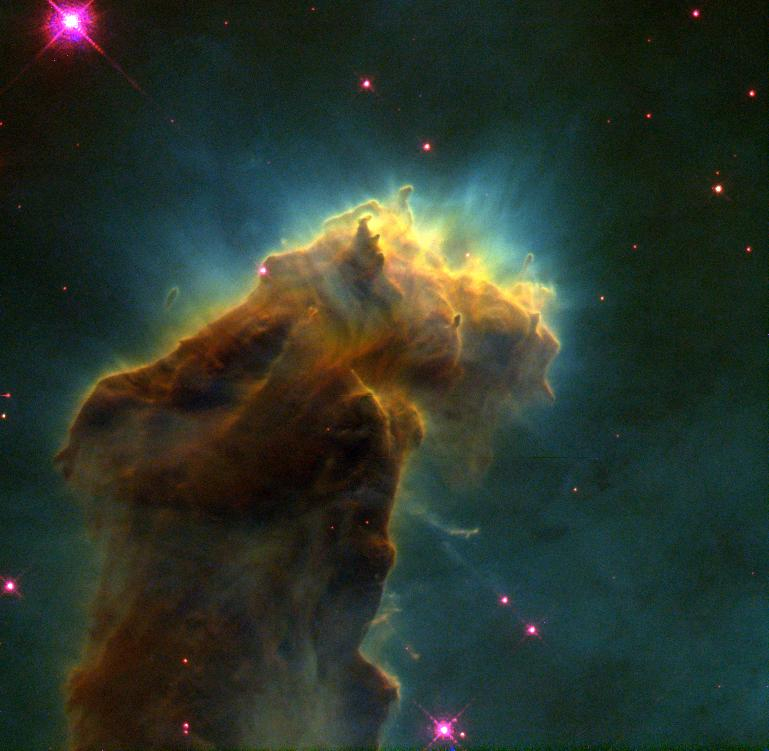
\includegraphics[width=0.9\linewidth]{eagle.jpg}
        \captionof{figure}{Nébula del águila. Fuente: HST}
    \end{minipage}
    \end{figure}
\end{frame}


\begin{frame}{Evolución estelar}
\begin{figure}
    \centering
    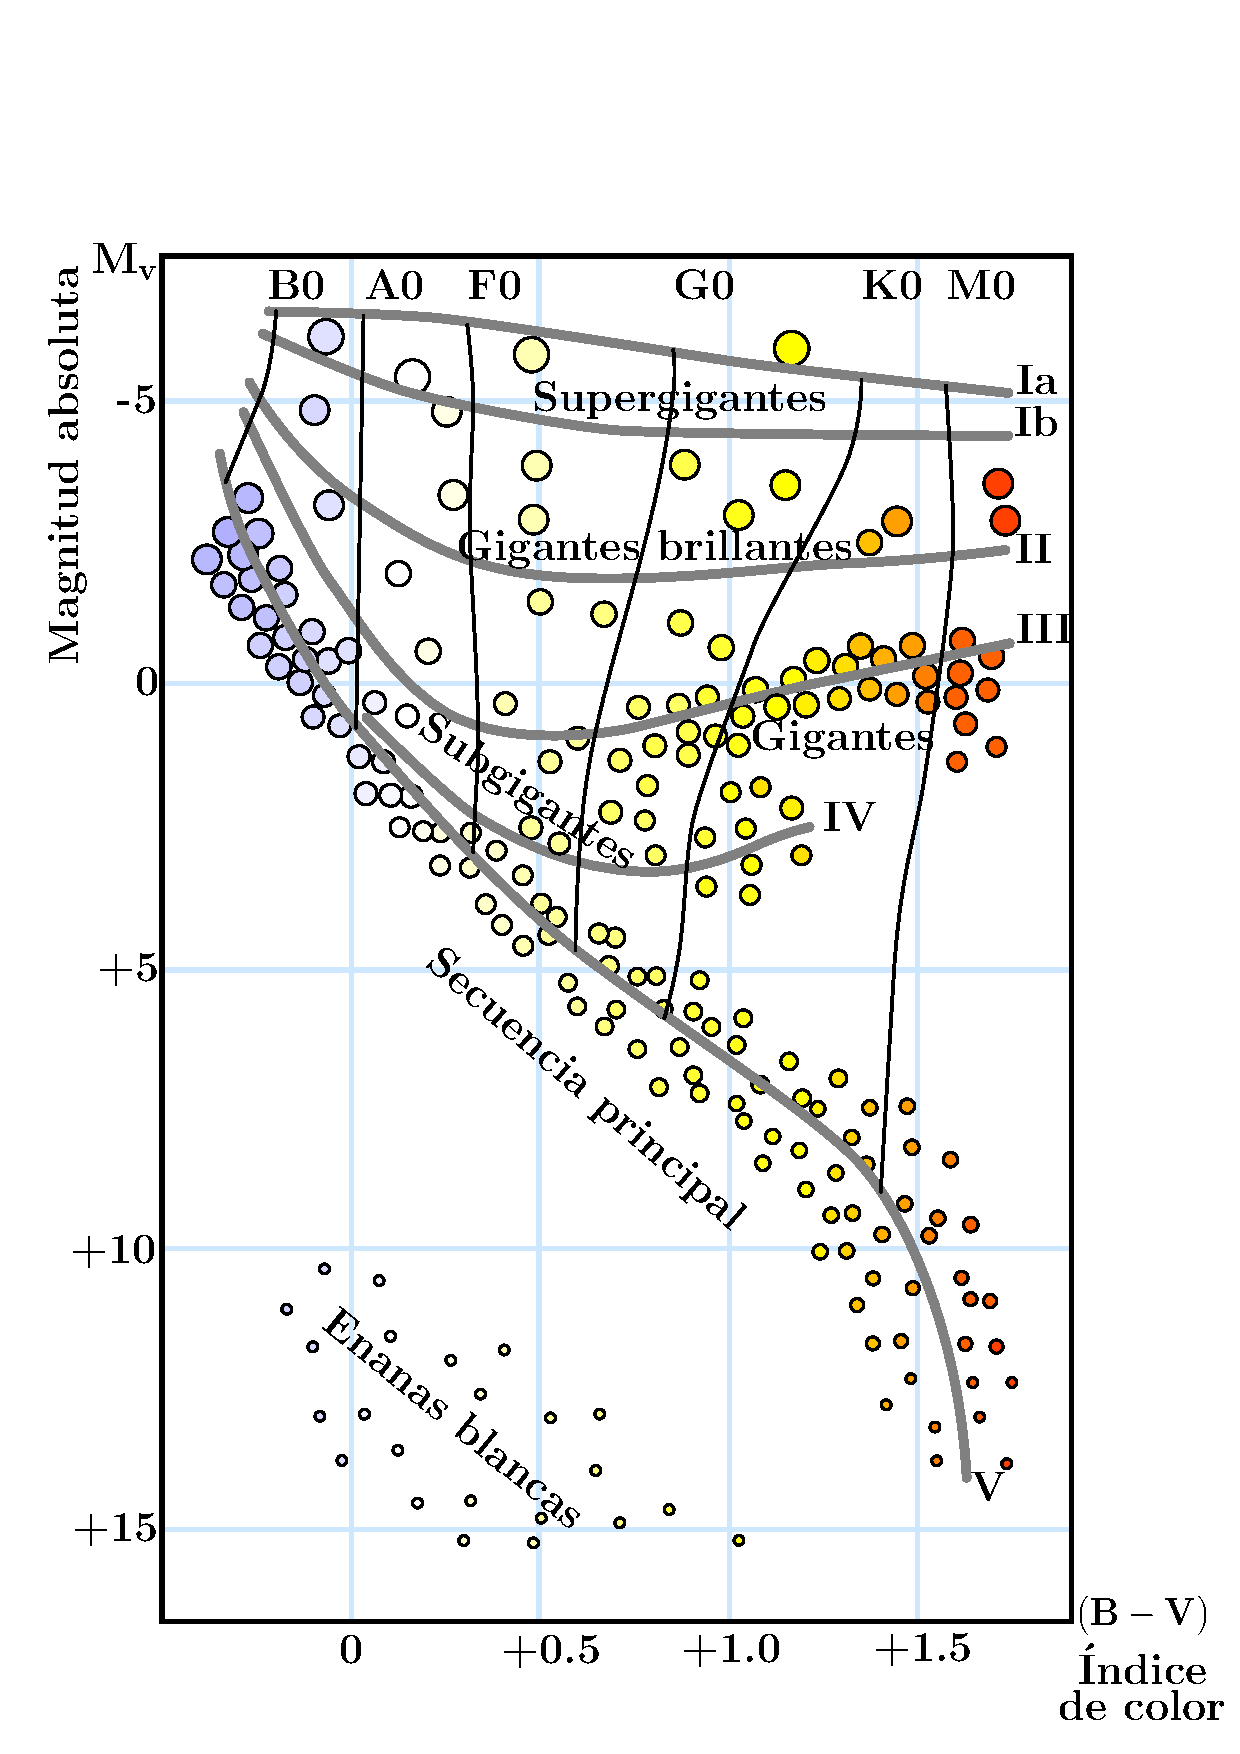
\includegraphics[width=0.55\linewidth,height=0.6\linewidth]{H-R_diagram.pdf}
    \caption{Diagrama de Hertzsprung-Russell. Fuente:}
\end{figure}
    
\end{frame}

\begin{frame}{}
    \begin{figure}
        \centering
        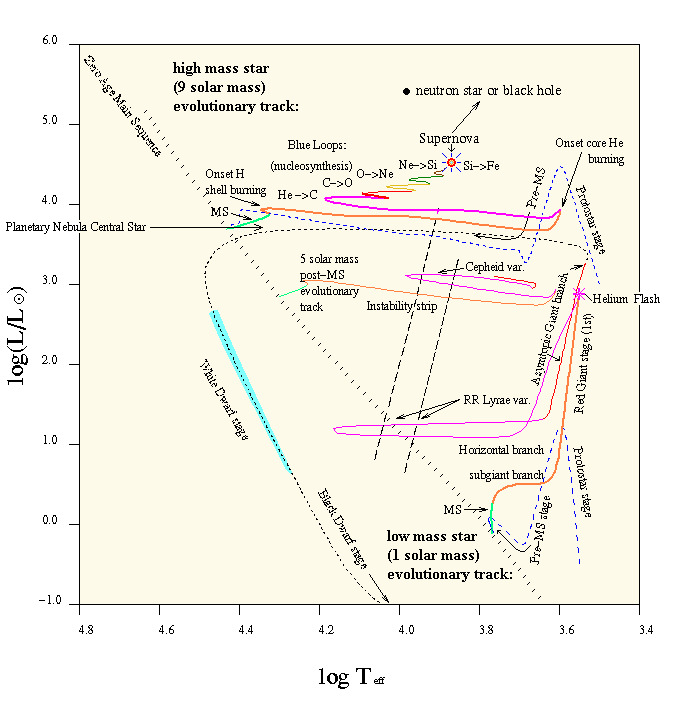
\includegraphics[width=0.7\linewidth]{evoltracks.jpg}
        \caption{Trayectorias evolutivas. Fuente:}
    \end{figure}
\end{frame}



\begin{frame}{Supernova}
    \begin{figure}
        \centering
        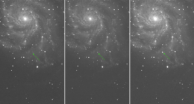
\includegraphics[width=0.95\linewidth]{disc.pdf}
        \caption{ SN 2011fe (Agosto 23, 24 y 25). Fuente: Supernova 2011fe from an Exploding Carbon-Oxygen White Dwarf Star. Nugent et al.}
    \end{figure}
\end{frame}

\begin{frame}{Energía liberada en una supernova}
\vspace{-0.85cm}
\begin{table}[]
\begin{adjustbox}{max width=\textwidth}
\begin{tabular}{ccccc}
\begin{tabular}[c]{@{}c@{}}Colapso del\\ núcleo de hierro\end{tabular} & $\longrightarrow$ & \begin{tabular}[c]{@{}c@{}}¿Liberación? de energía\\ potencial gravitacional\end{tabular} & $\longrightarrow$ & \begin{tabular}[c]{@{}c@{}}Explosión de \\ la estrella\end{tabular}
\end{tabular}
\end{adjustbox}
\end{table}

Si el núcleo tiene masa inicial $M_c$ y el radio pasa de $R_n$ a $R_{nc}$, con $R_{n}\gg R_{nc}$
\begin{equation}
        \Delta E _ { \mathrm { grav } } = - G M _ { c } ^ { 2 } \left( \frac { 1 } { R _ { n } } - \frac { 1 } { R _ { n c } } \right) \approx \frac { G M _ { c } ^ { 2 } } { R _ { n c } },
\end{equation}
usando $M _ { c } \approx 1.5 M _ { \odot }$, $R _ { c } \approx 10 ^ { 4 } \mathrm { km }$ y $R _ { n c } \approx 20 \mathrm { km }$
\begin{equation}
    \Delta E _ { \mathrm { grav } } \approx 3 \times 10^{46} \rm{J}.
\end{equation}
\end{frame}

\section{Objetos compactos}
\begin{frame}{Estrellas de neutrones}
    \begin{figure}
        \centering
        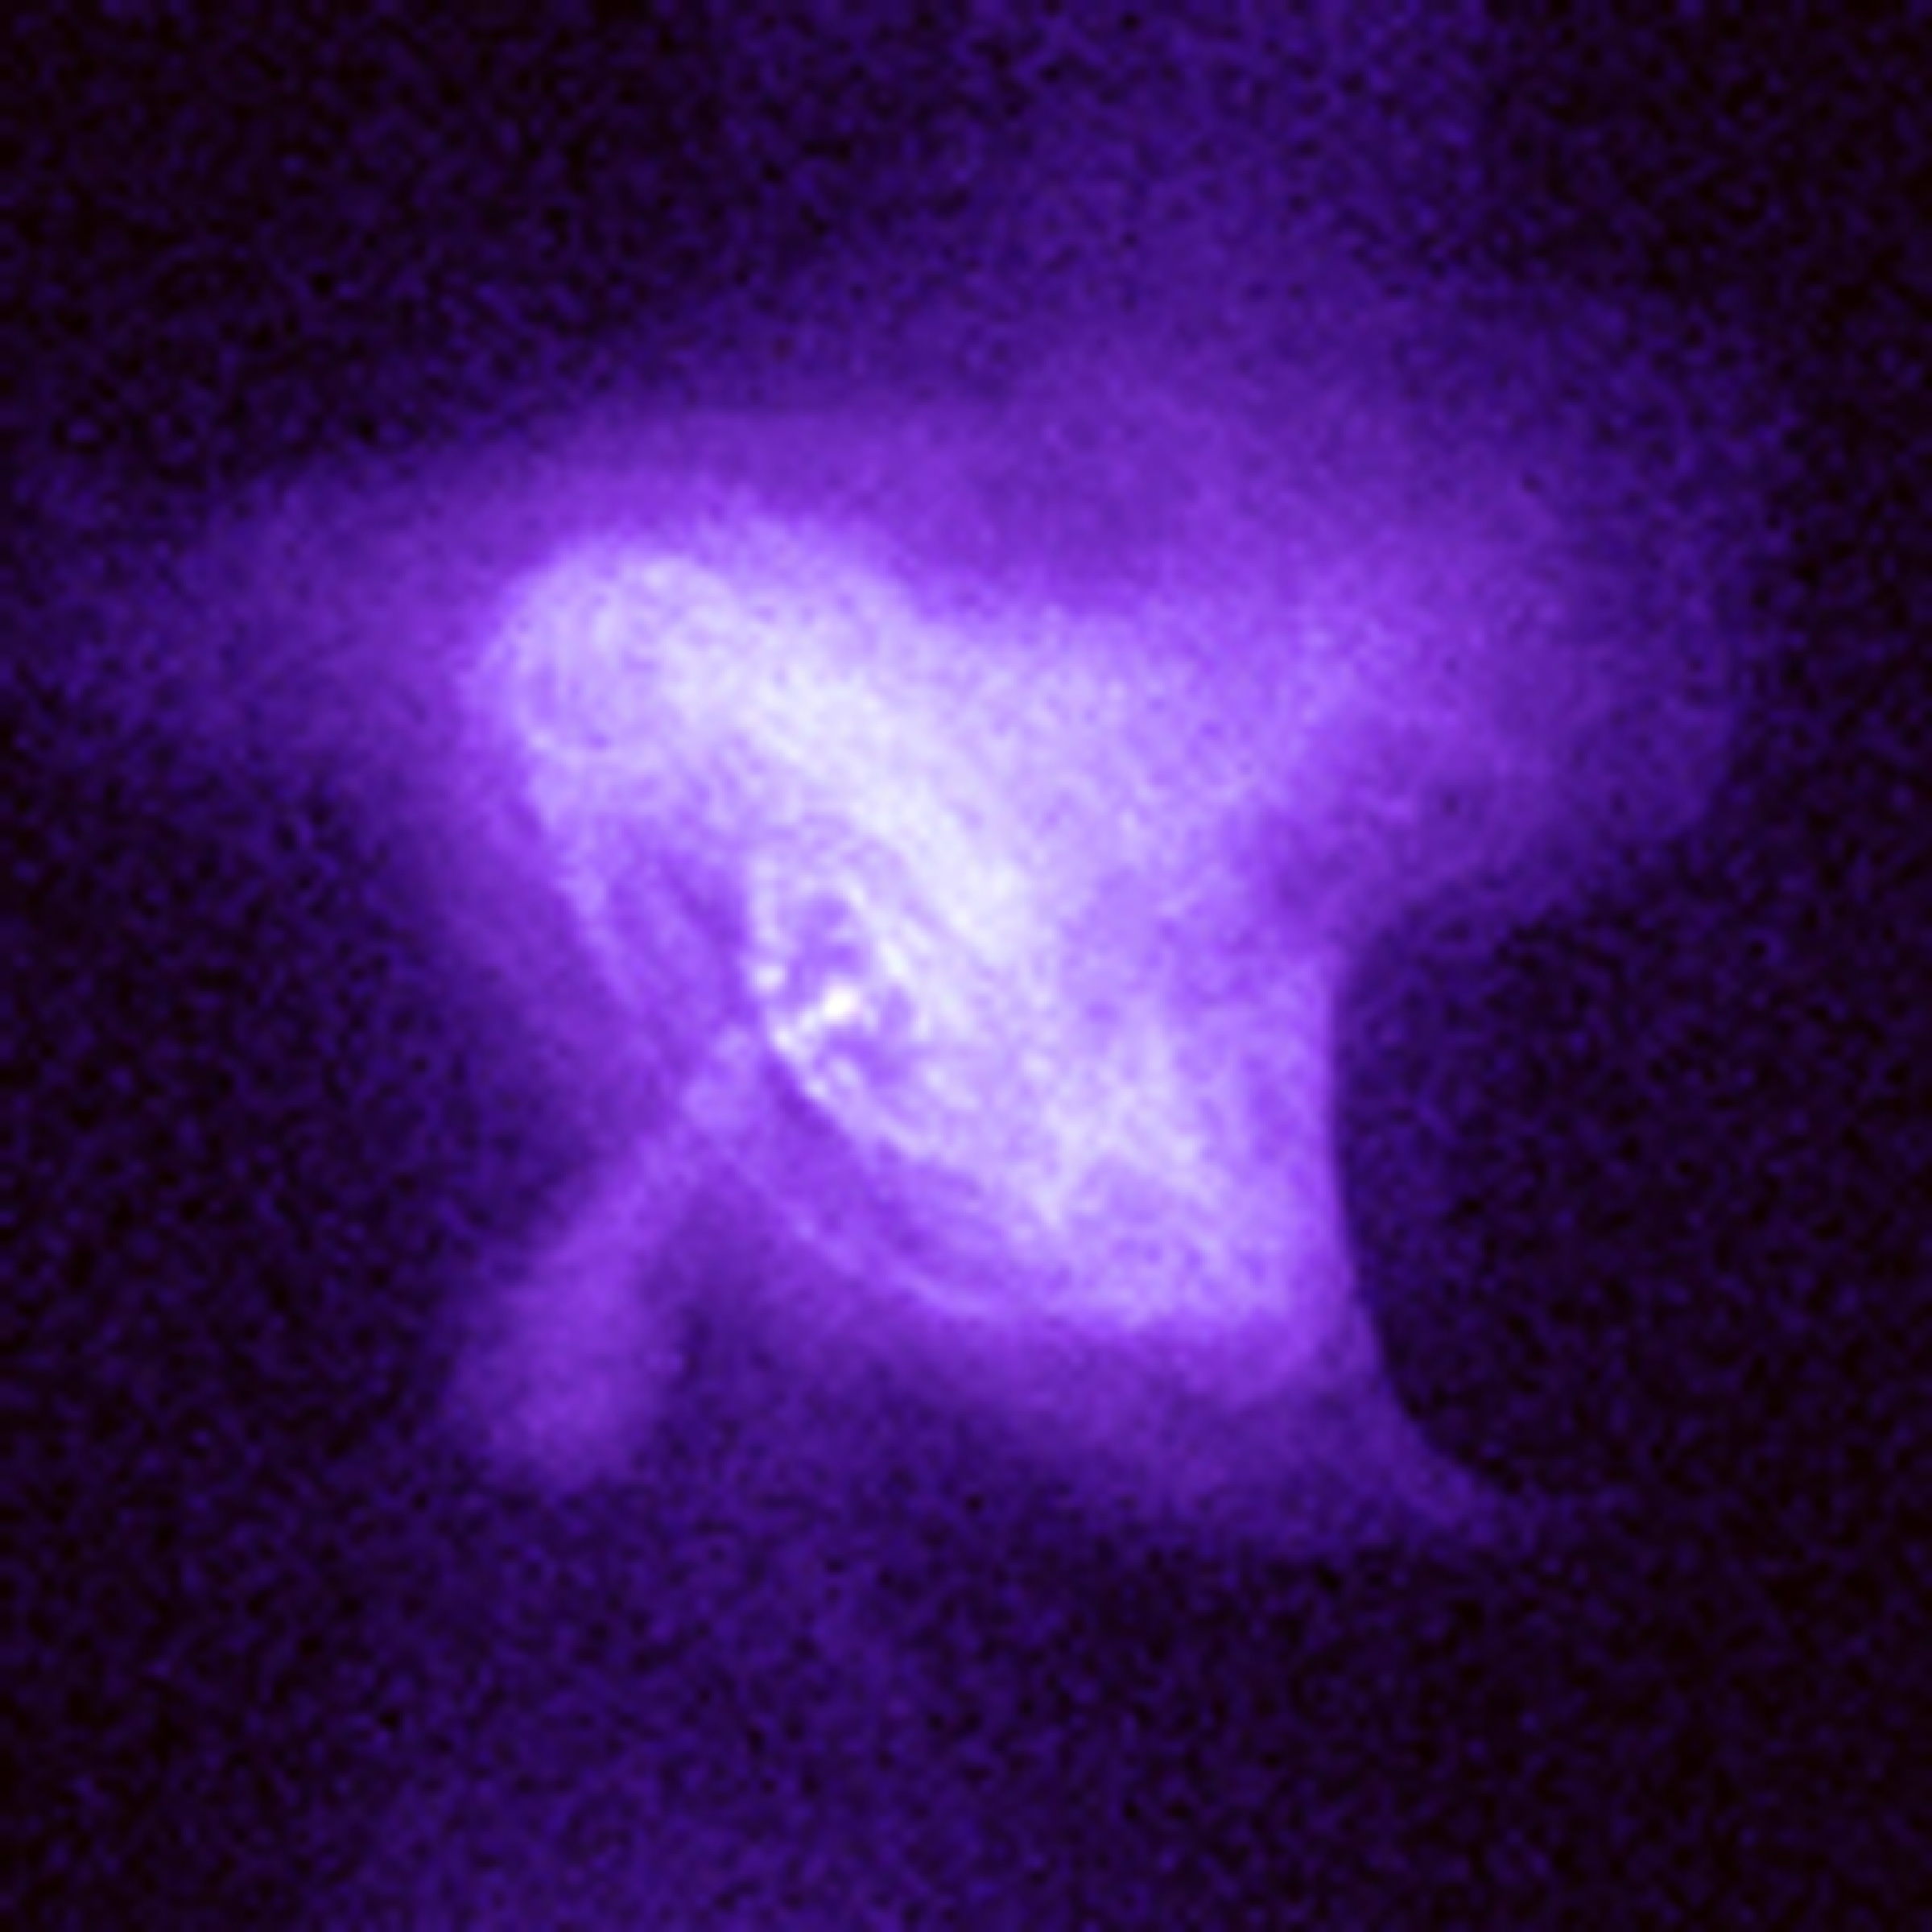
\includegraphics[width=0.6\linewidth]{crab.png}
        \caption{ Nebulosa del cangrejo, Rayos X. Fuente: Chandra X-Ray Observatory}
    \end{figure}
\end{frame}

\begin{frame}{Condiciones extremas}
    Modelo estándar de estrellas de neutrones:
    \begin{equation}
        M = 1.4 \,M _ { \odot },\quad R = 10 \,\mathrm { km }, \quad r_{\mathrm{g}}=4.13\,\mathrm{km},
    \end{equation}
    con esto
    \begin{equation}
        g = \frac{ G M }{ R^2\sqrt { 1 - r_{\mathrm{g}} / R }}=2.43 \times 10 ^ { 14 }\, \mathrm { cm\,s } ^ { - 2 },
    \end{equation}
    \begin{equation}
        \rho_{prom}=6.68\times 10^{17}\,\mathrm{g}\, \mathrm{cm^-3} > \rho_0= 2.3 \times 10^{14}\,\mathrm{g}\, \mathrm{cm^{-3}}.
    \end{equation}
\end{frame}

\section{Estructura Estelar}

\begin{frame}{Equilibrio hidrostático}
    \begin{wrapfigure}{l}{0.4\linewidth}
        \centering
        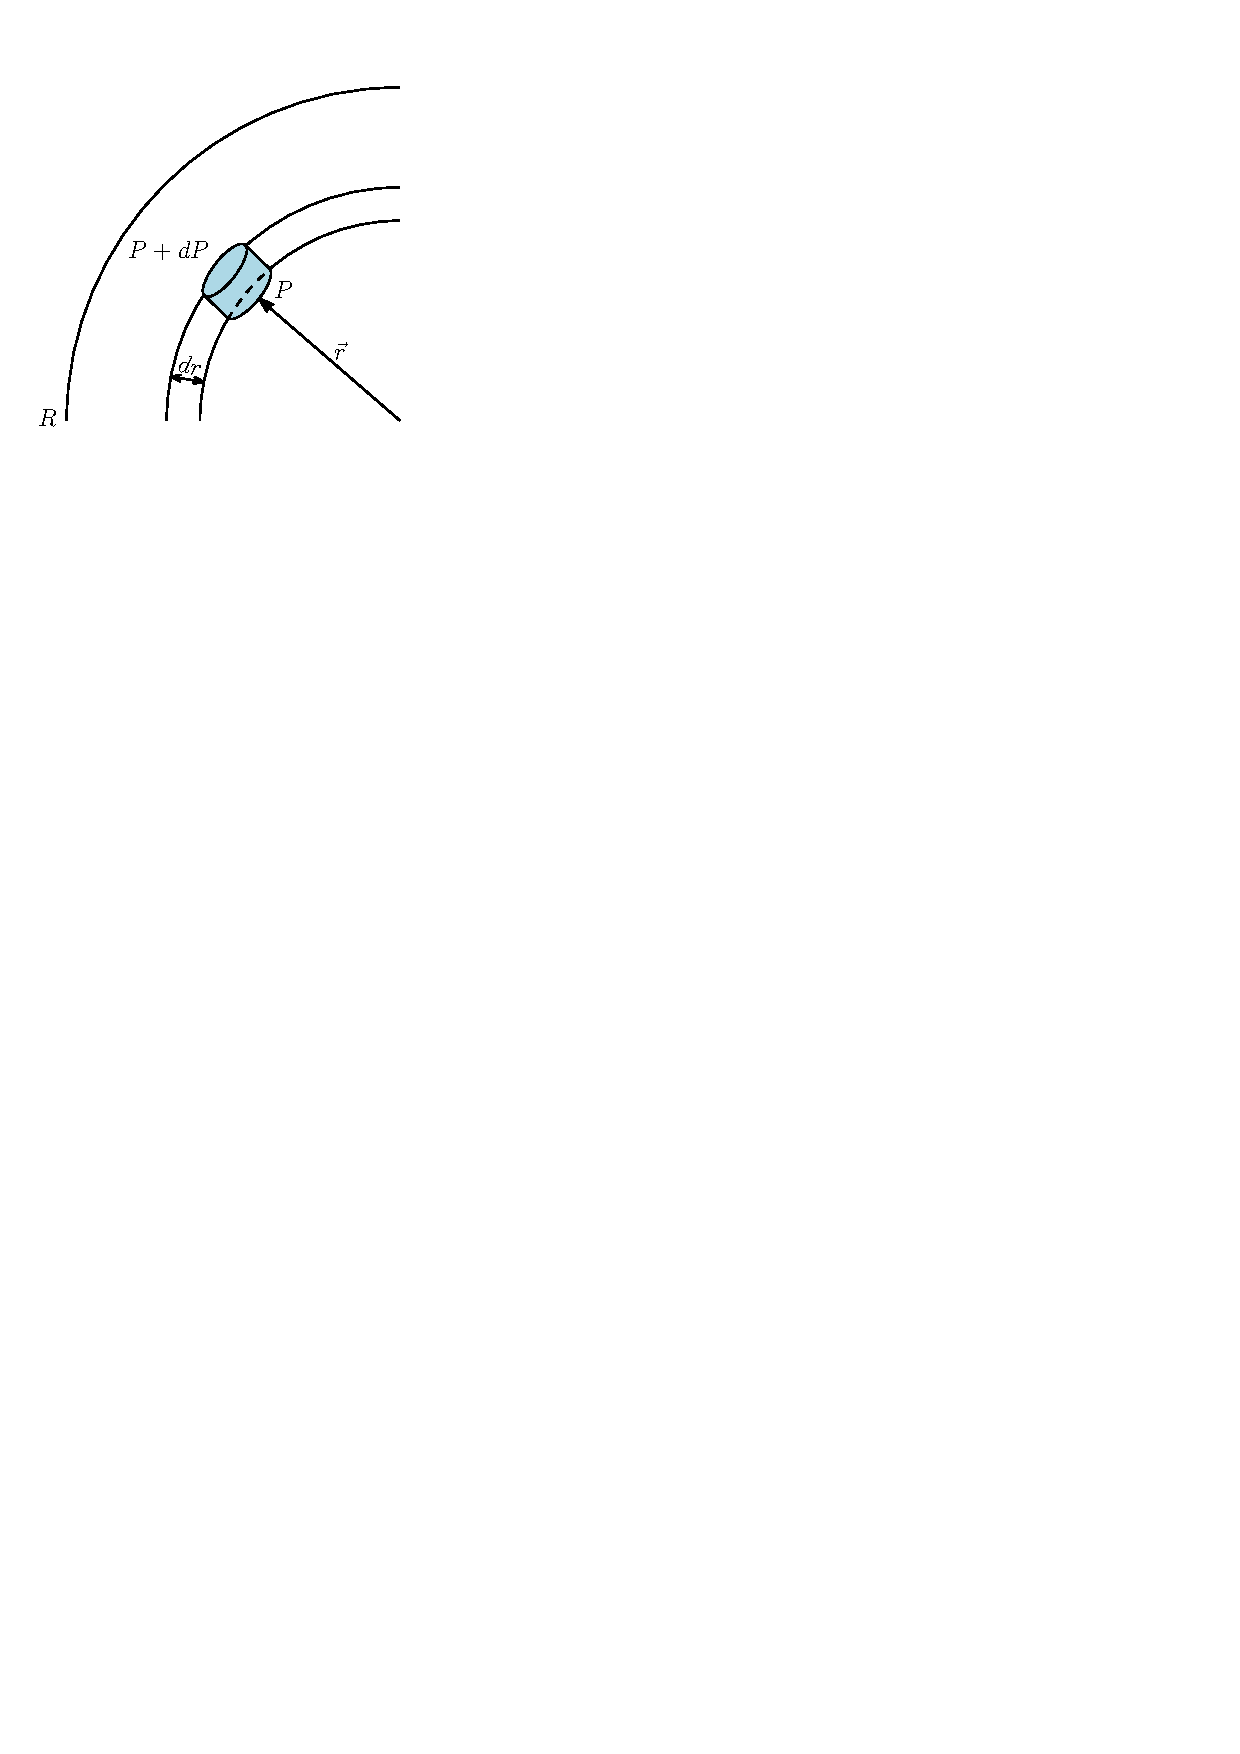
\includegraphics[width=\linewidth]{stellarnewton.pdf}
    %\caption{Caption}
    \end{wrapfigure}
    Fuerza por diferencia de presión
    \begin{equation*}
        F _ { \text{Pelem} } = - d P d A.
    \end{equation*}
    Fuerza ejercida por la masa interior
    \begin{equation*}
        F_{atracc}=\frac{G m(r)\rho \dd{A} \dd{r}}{r^2}.
    \end{equation*}
    Para el equilibrio requerimos
    \begin{equation}
        -\dd{P}\dd{A} =\frac{G m(r)\rho \dd{A} \dd{r}}{r^2}.
    \end{equation}
\end{frame}

\begin{frame}{Ecuaciones de estructura newtonianas}
    Masa encerrada entre dos cascarones separados infinitesimalmente
    \begin{equation*}
        \dd{m(r)}=4\pi r^2\rho \dd{r}.
    \end{equation*}
    Re escribiendo los dos resultados:
    \vspace{0.3cm}
    \begin{subequations}
    \begin{empheq}[left= \textbf{Ecuaciones de estructura} \empheqlbrace]{align}
         \dv{m}{r} &=4\pi r^2 \rho, \\
        \dv{P}{r} &= - \frac { G m  } { r ^ { 2 } } \rho.
    \end{empheq} 
    \end{subequations}
\end{frame}



%\begin{frame}{¿Por qué Relatividad General?}
 %   ...
%\end{frame}

\begin{frame}{Algo de Relatividad General}
    \begin{figure}
        \centering
        
\includegraphics[page=1,scale=0.65]{GR.pdf}
    \end{figure}
\end{frame}

\begin{frame}{Algo de Relatividad General}
    \begin{figure}
        \centering
        
\includegraphics[page=2,scale=0.65]{GR.pdf}
    \end{figure}
\end{frame}

\begin{frame}{Algo de Relatividad General}
    \begin{figure}
        \centering
        
\includegraphics[page=3,scale=0.65]{GR.pdf}
    \end{figure}
\end{frame}

\begin{frame}{Algo de Relatividad General}
    \begin{figure}
        \centering
        
\includegraphics[page=4,scale=0.65]{GR.pdf}
    \end{figure}
\end{frame}

\begin{frame}{Solución exterior}
    De las ecuaciones de Einstein,
    \begin{equation}
        G _ { \mu } ^ { \nu } = R _ { \mu } ^ { \nu } - \frac { 1 } { 2 } \delta _ { \mu } ^ { \nu } R = 0,
    \end{equation}
    se obtiene
    \begin{equation}
        e ^ { 2 \nu } = 1 - \frac { 2 M } { r }\quad \text{y}\quad - e ^ { 2 \lambda } = - e ^ { - 2 \nu } = - \left( 1 - \frac { 2 M } { r } \right) ^ { - 1 },
    \end{equation}
    la métrica para $r<R$ será entonces
    \begin{equation}
        \dd{s} ^ { 2 } =  \left( 1 - \frac { 2 M } { r } \right) \dd{t} ^ { 2 } - \left( 1 - \frac { 2 M } { r } \right) ^ { - 1 } \dd{r} ^ { 2 }  - r ^ { 2 }\left( \dd{\theta} ^ { 2 } +  \sin ^ { 2 } \theta \dd{\phi} ^ { 2 } \right).
    \end{equation}
    
    \hyperlink{extsol}{\beamerbutton{Derivación}}
\end{frame}

\begin{frame}{Solución interior}
    Modelando la estrella como un fluido ideal (\hyperlink{idealfluid}{\beamerbutton{ver más}})
    \begin{equation}
         T _ { 0 } ^ { 0 } = \rho(r) , \quad T _ { i } ^ { i } = - P(r) \quad ( i=1,2,3 ),
    \end{equation}
    las ecuaciones de Einstein,
    \begin{equation}
        G _ { \mu } ^ { \nu } = R _ { \mu } ^ { \nu } - \frac { 1 } { 2 } \delta _ { \mu } ^ { \nu } R = 8 \pi T _ { \mu } ^ { \nu },
    \end{equation}
    se convierten en 
    \vspace{-0.6cm}
    \begin{subequations}
    \begin{empheq}[left= \textbf{Ecuaciones de TOV} \empheqlbrace]{align}
         \dv{m}{r} =&\, 4 \pi r ^ { 2 } \rho, \\
        \dv{P}{r} =& - \frac { ( P  + \rho ) \left( m  + 4 \pi r ^ { 3 } P \right) } { r ( r - 2 m ) },
    \end{empheq}
    \vspace{-0.7cm}
    \begin{align}
        \quad\quad\,\,\,\,\,\,\dv{\nu}{r} = \frac { m  + 4 \pi r ^ { 3 } P  } { r ( r - 2 m  ) },
    \end{align}
    \end{subequations}
    \hyperlink{intsol}{\beamerbutton{Derivación}}
\end{frame}

\begin{frame}{}
    donde se definió la función de masa o masa de Misner
    \begin{equation}
        m ( r ) \equiv 4 \pi \int _ { 0 } ^ { r } \rho ( r ) r ^ { 2 }     \dd{r}. \quad \hyperlink{masa}{\beamerbutton{Nota}}
    \end{equation}
    
    \vspace{0.7cm}
    
    \alert{Interpretación física}
    
    Re-escribiendo el gradiente de presión 
    \begin{equation}
        \dv{P}{r} =  - \frac { G m } { r ^ { 2 } } \rho \left[ 1 + \frac { P  } {c ^ { 2 } \rho  } \right] \left[ 1 + \frac { 4 \pi r ^ { 3 } P } { m c ^ { 2 } } \right]  \left[ 1 - \frac { 2 G m } { c ^ { 2 } r } \right] ^ { - 1 }.
    \end{equation}
\end{frame}

\begin{frame}{Resolviendo el sistema}
    Las ecuaciones de TOV son un IVP
    \begin{table}[]
        \begin{tabular}{ccc}
            \parbox{3cm}{\begin{equation*}\dv{m}{r} =\, 4 \pi r ^ { 2 }\end{equation*}}       & $\longrightarrow$                     & $m(0)=0$ \\
            \parbox{5cm}{\begin{equation*}
                \dv{P}{r} = - \frac { ( P  + \rho ) \left( m  + 4 \pi r ^ { 3 } P \right) } { r ( r - 2 m ) }
            \end{equation*}}     &       $\longrightarrow$      &       $P(0)=P_c$ \\
            \parbox{4cm}{\begin{equation*}
                \dv{\nu}{r} = \frac { m  + 4 \pi r ^ { 3 } P  } { r ( r - 2 m  ) }
            \end{equation*}}  &       $\longrightarrow$      &       $\nu(0)=0$
        \end{tabular}
    \end{table}
    \alert{Pero...} necesitamos una ecuación de estado $P(\rho)$ .
\end{frame}

\section{Composición de estrellas de neutrones}
\begin{frame}{Composición de una estrella de neutrones}
    \begin{figure}
        \centering
        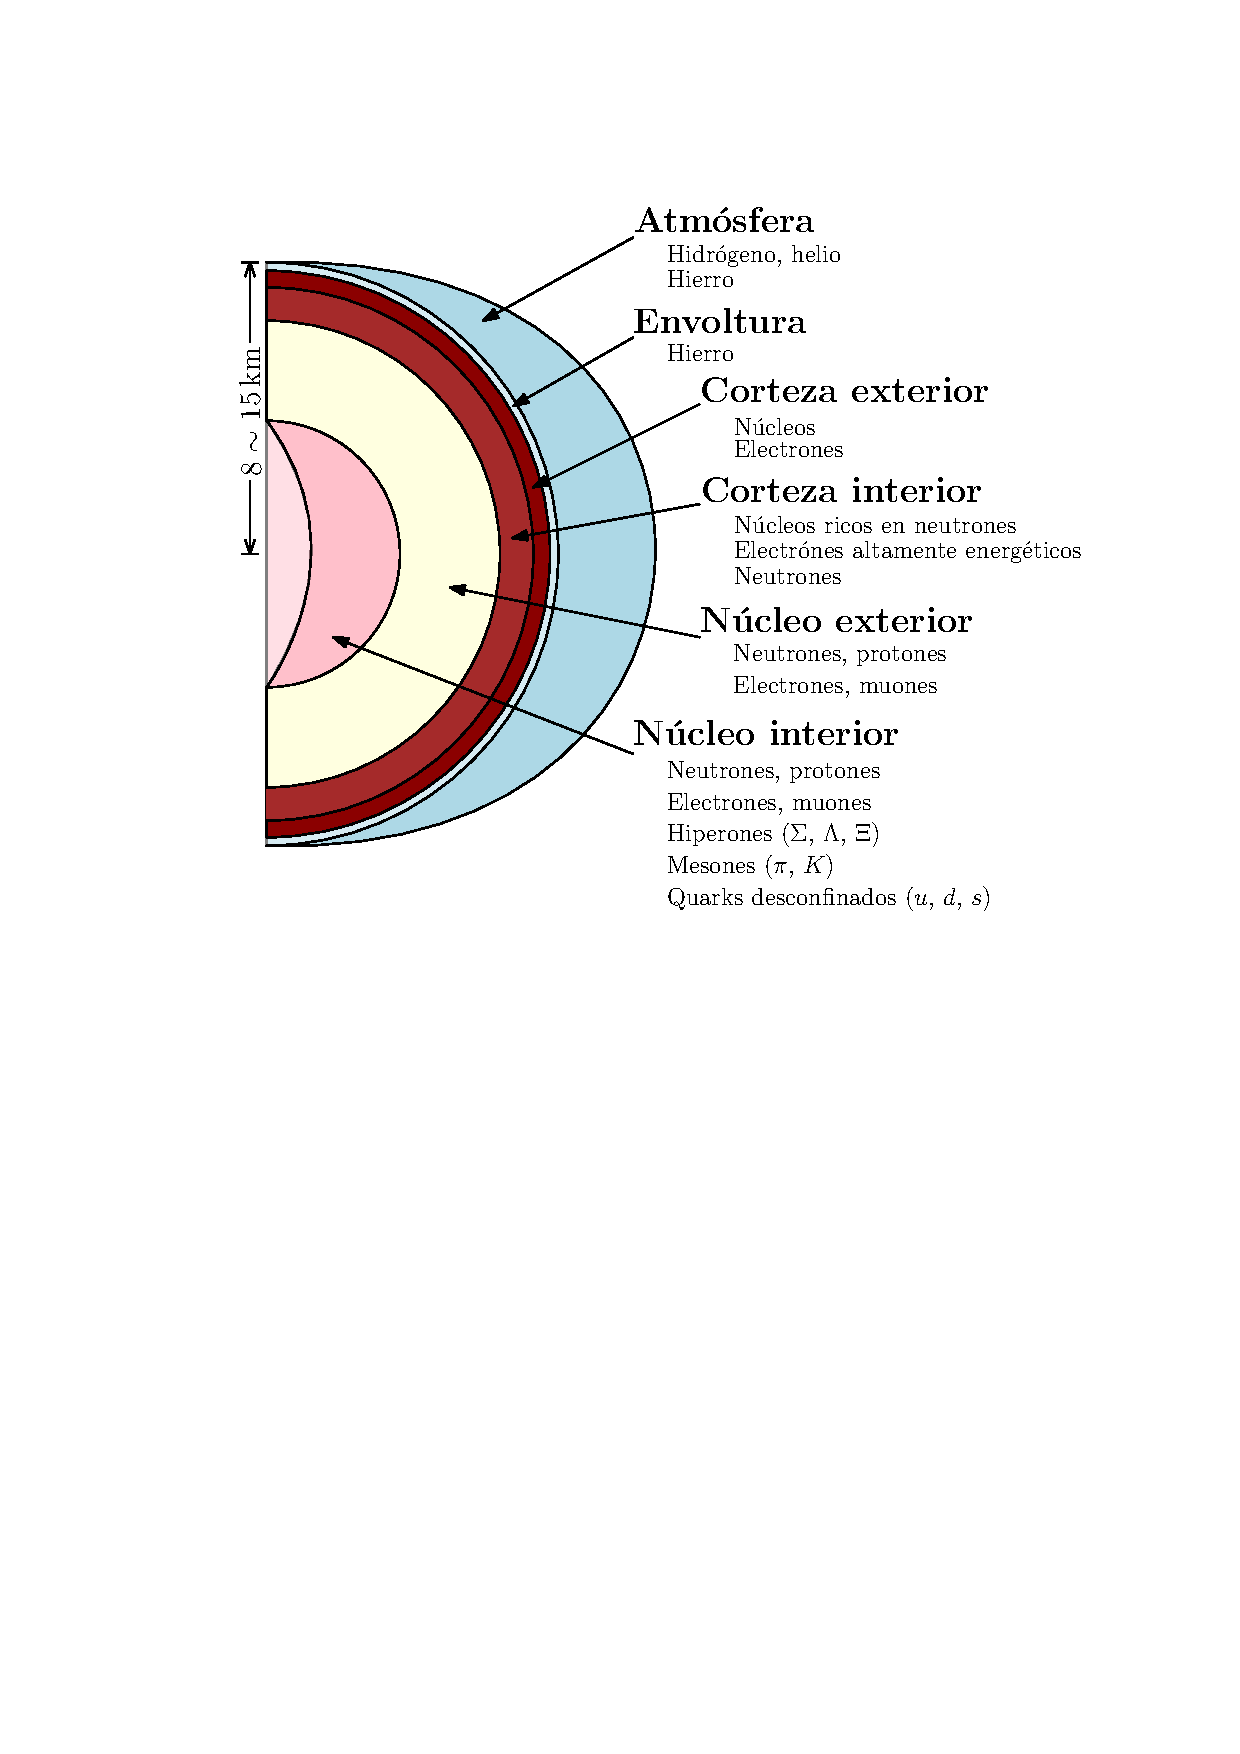
\includegraphics[width=0.7\linewidth]{neutronstar.pdf}
    \end{figure}
\end{frame}

\begin{frame}{Una variedad de fases}
    \begin{figure}
        \centering
        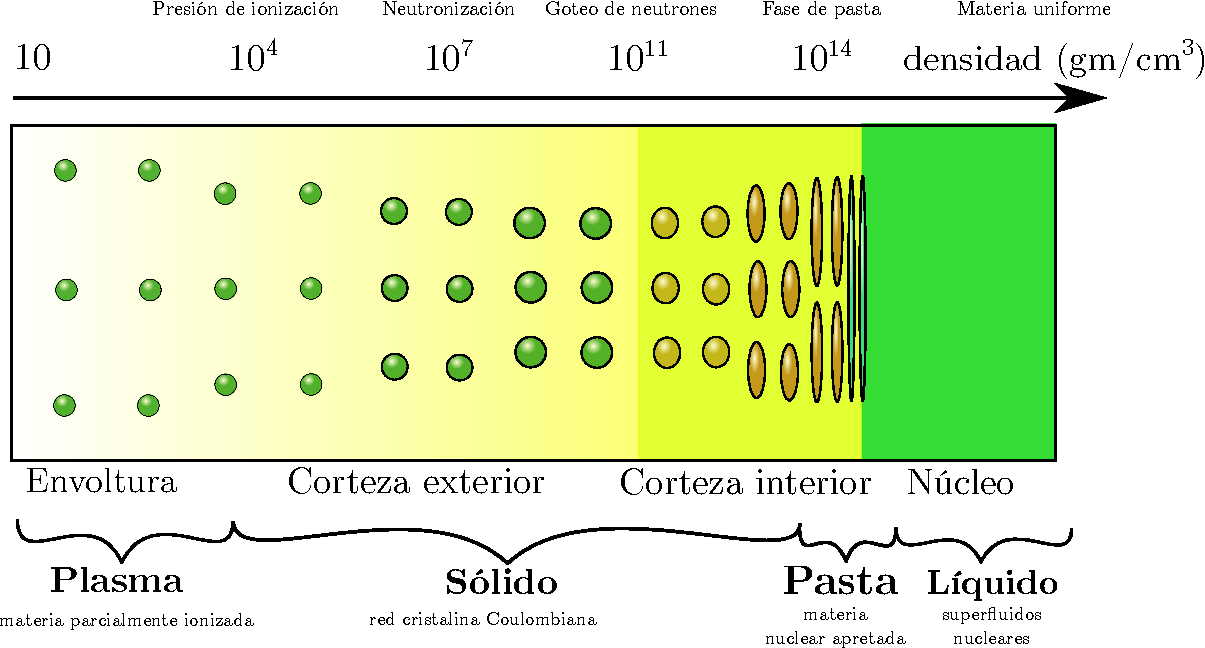
\includegraphics[width=\linewidth]{Density.pdf}
    \end{figure}
\end{frame}

\begin{frame}{Ecuación de estado}
    \begin{textblock*}{0.5pt}(60mm,20mm)
    ALF
    \end{textblock*}
    \begin{textblock*}{0.5pt}(50mm,25mm)
    AP
    \end{textblock*}
    \begin{textblock*}{0.5pt}(70mm,25mm)
    WFF
    \end{textblock*}
    \begin{textblock*}{0.5pt}(45mm,30mm)
    SQM
    \end{textblock*}
    \begin{textblock*}{0.5pt}(75mm,30mm)
    PAL
    \end{textblock*}
    \begin{textblock*}{0.5pt}(45mm,35mm)
    BBB
    \end{textblock*}
    \begin{textblock*}{0.5pt}(75mm,35mm)
    NL
    \end{textblock*}
    \begin{textblock*}{0.5pt}(75mm,40mm)
    BSK
    \end{textblock*}
    \begin{textblock*}{0.5pt}(70mm,45mm)
    ENG
    \end{textblock*}
    \begin{textblock*}{0.5pt}(65mm,50mm)
    FPS
    \end{textblock*}
    \begin{textblock*}{0.5pt}(60mm,55mm)
    GNH
    \end{textblock*}
    \begin{textblock*}{0.5pt}(60mm,60mm)
    SLy
    \end{textblock*}
    \begin{textblock*}{0.5pt}(60mm,65mm)
    MPA
    \end{textblock*}
    \begin{textblock*}{0.5pt}(60mm,70mm)
    MS
    \end{textblock*}
    \begin{textblock*}{0.5pt}(60mm,75mm)
    NJL
    \end{textblock*}
    \begin{textblock*}{0.5pt}(60mm,85mm)
    QMC
    \end{textblock*}

\end{frame}

\section{Condiciones de aceptabilidad}
\begin{frame}{Condicionando los posibles modelos}
    \begin{itemize}
        \item \textbf{C1} \\
            Las funciones métricas son positivas y deben ser finitas y libres de singularidades en el
            interior de la estrella.
        \item \textbf{C2 Acomplamiento}  \\
            \begin{equation}
                e ^ { -2 \lambda(R) } =  e ^ {  2 \nu(R) } =  1 - \frac { 2 M } { R }.
            \end{equation}
        \item \textbf{C3 Corrimiento al rojo} \\
            \begin{equation}
                z(r)\equiv e^{-\nu(r)}-1,
            \end{equation}
            debe disminuir con el incremento de r.
    \end{itemize}
\end{frame}

\begin{frame}{}
    \begin{itemize}
        \item \textbf{C4} \\
        La densidad de energía y la presión deben ser positivas dentro de la estrella.
        \item \textbf{C5} \\
        La densidad de energía y la presión deben alcanzar un máximo en el centro ($\rho'(0)=P'(0)=0$) y deben decrecer monótonamente hacia afuera.
        \item \textbf{C6} \\
        La solución debe satisfacer la condición de energía dominante (DEC) $\rho \geq |P|$.
        \item \textbf{C7 Causalidad} \\ 
        \begin{equation}
            v^2=\dv{P}{\rho}\leq 1.
        \end{equation}
    \end{itemize}
\end{frame}


\begin{frame}{}
    \begin{itemize}
        \item \textbf{C8 Estabilidad ante pulsaciones radiales I} \\
            \begin{equation}
                \Gamma = \frac { \rho + P  } { P } \dv{P}{\rho} \geq \frac{4}{3}.
            \end{equation}
        \item \textbf{C9 Estabilidad ante cracking} \\
            \begin{equation}
                \dv{P}{r}\leq 0.
            \end{equation}
        \item \textbf{C10 Estabilidad ante pulsaciones radiales II} \\
            \begin{equation}
                \frac { \partial M } { \partial \rho _ { c } } > 0.
            \end{equation}
        \item \textbf{C11 Estabilidad ante movimientos convectivos} \\
            \begin{equation}
                \dv[2]{\rho }{r} \leq 0.
            \end{equation}
    \end{itemize}
\end{frame}

\section{Planteamiento del problema}
\begin{frame}[plain]{Planteamiento del problema}
    \vspace{1cm}
    \begin{figure}
        \centering
        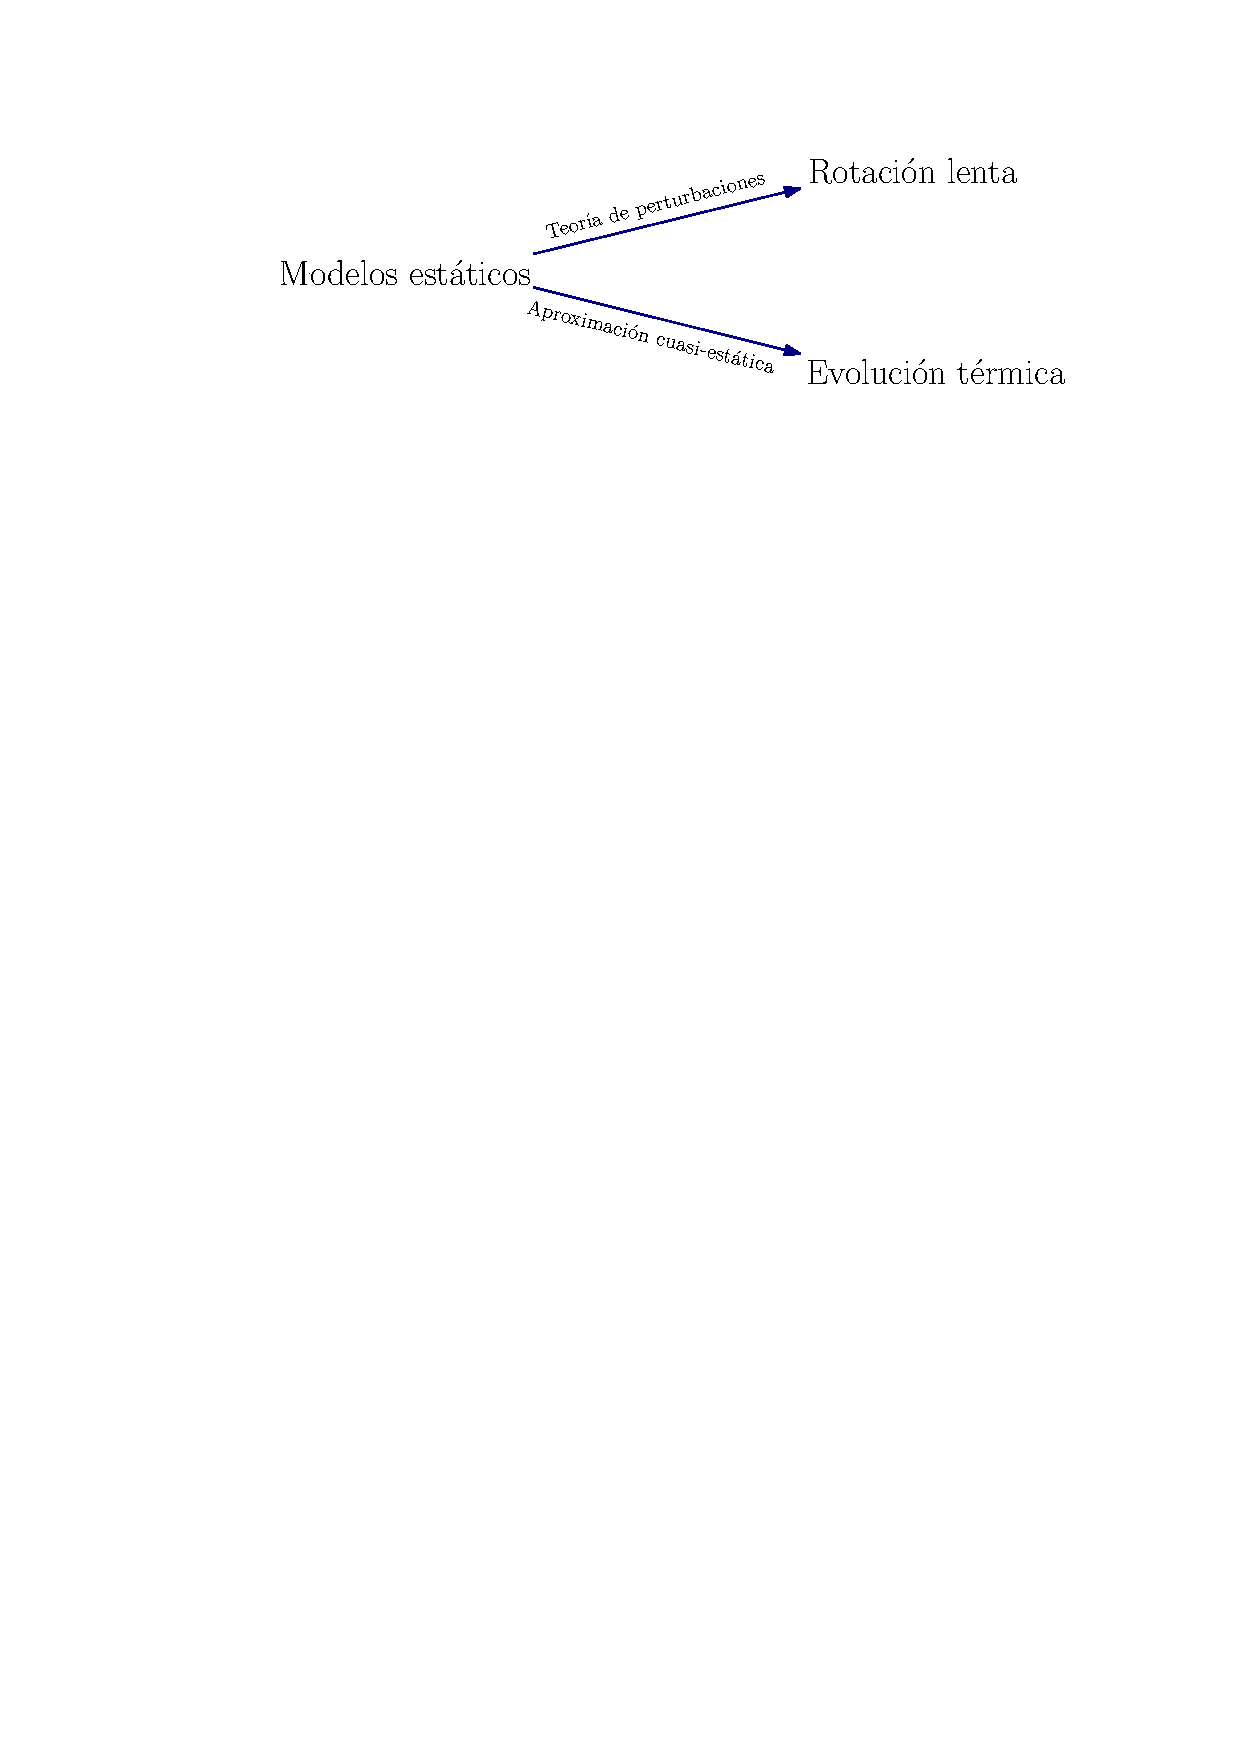
\includegraphics[width=0.9\linewidth]{staticm.pdf}
    \end{figure}
    \pause
    \vspace{1cm}
    ¿Cómo escoger entre la variedad de ecuaciones de estado al construir modelos estáticos?
    \pause
    \alert{Condiciones de aceptabilidad}
    
    \begin{pgfpicture}{0}{0}{12.8cm}{3.2cm}
    \pgfputat{\pgfxy(10.55,1.38)}{\pgfbox[left,base]{ %
      \scriptsize{\insertframenumber{}/\inserttotalframenumber}}}
    \end{pgfpicture}
\end{frame}

\section{Objetivos}

\begin{frame}[plain]{Objetivos}
    \vspace{0.8cm}
    \textbf{\large{Objetivo general}}\\ \vspace{0.3cm}
    Determinar si los modelos de estrellas de neutrones obtenidos con las ecuaciones de
    estado encontradas en la literatura son estables ante convección.\\
    \vspace{0.5cm}
    \textbf{\large{Objetivos específicos}}\\\vspace{0.3cm}
    \begin{enumerate}
        \item Obtener modelos de estrellas de neutrones en equilibrio para las distintas ecuaciones de estado.
    \item Descartar los modelos que no cumplan las condiciones C1-C10.
    \item Evaluar a los modelos restantes ante convección adiabática usando el criterio C11.
    \end{enumerate}
    \begin{pgfpicture}{0}{0}{12.8cm}{3cm}
    \pgfputat{\pgfxy(10.55,1.38)}{\pgfbox[left,base]{ %
      \scriptsize{\insertframenumber{}/\inserttotalframenumber}}}
    \end{pgfpicture}
    
\end{frame}





\section{Metodología}
\begin{frame}[plain]{Metodología}
    \vspace{0.5cm}
    \begin{enumerate}
    \item Reunir ecuaciones de estado para la materia densa tabuladas de la literatura, necesarias para resolver las ecuaciones de TOV.
    \item Interpolar las ecuaciones de estado manera óptima, explorando las distintas posibilidades.
    \item Resolver las ecuaciones de TOV numéricamente usando una ecuación de estado interpolada, para obtener modelos de estrellas de neutrones estáticas. Se usará en lo posible el ecosistema de software de código abierto para cómputo científico (SciPy) de Python.
    \item Obtener las derivadas $\dv{P}{\rho}$ ,  $\dv{P}{r}$, $\dv[2]{P}{r}$, $\dv{\rho}{r}$ y $\dv[2]{\rho}{r}$, numéricamente. Esto permitirá evaluar la mayoría las condiciones de aceptabilidad física. 
\end{enumerate}

    \begin{pgfpicture}{0}{0}{12.8cm}{2.8cm}
    \pgfputat{\pgfxy(10.55,1.38)}{\pgfbox[left,base]{ %
      \scriptsize{\insertframenumber{}/\inserttotalframenumber}}}
    \end{pgfpicture}

\end{frame}

\begin{frame}{}
    \begin{enumerate}
    \setcounter{enumi}{4}
        \item Variar la densidad central $\rho_c$ en las condiciones iniciales para obtener la familia de configuraciones en equilibrio asociada a la ecuación de estado y graficar las relaciones $M$-$R$ y $M$-$\rho_c$. Usado estos diagramas se puede identificar la masa máxima de la familia de soluciones y evaluar la condición C10, respectivamente.
    \end{enumerate}
\end{frame}

\begin{frame}[plain,noframenumbering]{Bibliografía}

\end{frame}


\begin{frame}[plain,noframenumbering,label=extsol]{Derivación de la solución exterior de Schwarzschild}
    
\end{frame}

\begin{frame}[plain,noframenumbering, label=idealfluid]{Fluidos Ideales}
    
\end{frame}

\begin{frame}[plain,noframenumbering,label=intsol]{Derivación de la solución interior: ecuaciones de TOV}
    \begin{align}
        G _ { 0 } ^ { 0 } =& -e ^ { - 2 \lambda } \left( \frac { 1 } { r ^ { 2 } } - \frac { 2 \lambda ^ { \prime } } { r } \right) + \frac { 1 } { r ^ { 2 } } = 8 \pi  \rho ( r ),  \\
         G _ { 1 } ^ { 1 } =& -e ^ { - 2 \lambda } \left( \frac { 1 } { r ^ { 2 } } + \frac { 2 \nu ^ { \prime } } { r } \right) + \frac { 1 } { r ^ { 2 } } = -8 \pi  P ( r ),  \\
         G _ { 2 } ^ { 2 } =& -e ^ { - 2 \lambda } \left( \nu ^ { \prime \prime } + \nu ^ { \prime 2 } + \lambda ^ { \prime } \nu ^ { \prime } + \frac { \nu ^ { \prime } - \lambda ^ { \prime } } { r } \right) = -8 \pi  P ( r ),  \\
          G _ { 3 } ^ { 3 } =& G _ { 2 } ^ { 2 } = -8 \pi  P ( r ).
    \end{align}
\end{frame}

\begin{frame}[plain,noframenumbering,label=masa]{Sobre la función de masa}
    $m(r)$ \textbf{NO} es la suma de las energías propias de los elementos de fluido
    \begin{equation}
        4 \pi \int _ { 0 } ^ { r } \rho ( r ) e^{2\lambda}r ^ { 2 }     \dd{r}.
    \end{equation}
\end{frame}

\end{document}